%!TEX root = thesis.tex
%% %% ***************** Research materials and methods *****************

%% ************************************************ 3 ************************************************

\section{Research material and methods}\label{sec:research-material-and-methods}
%\section{Tutkimusaineisto ja -menetelmät}

In the next section
we explain in more detail
what the data used in the study
consists of
and what methods were used
in attempt to answer the research goals.
The content of the section is briefly described below,
and the steps of the research are explained. %% TODO: Better phrasing

The data in the research is mainly made of two parts.
The most important part is, obviously,
the log data produced by the numerous RPA processes.
The second part complementing the study
is the support ticket data written by clerks of customer banks.
In order to use the data safely in the cloud environment
it was necessary to sanitize the data
from any sensitive information.
This was done by anonymizing the log data
and using only timestamps from the support tickets.

After confirming the results of anonymization,
the data was preprocessed into a better form
to make it more usable by algorithms.
More processing was done inside the pipeline
as ML Studio offered several usable components for this
but main cleaning was easier and to execute in local environment.
This was also done with PowerShell scripting.

ML pipeline was created in Azure ML Studio
and several ML algorithms were compared
in order to find the most feasible for our goal in mind.
ML training was organized in two different phases
in order to find the relation between
log anomalies and technical tickets.

Finally,
the results of the trained algorithms
were validated against newly acquired production data
in order to estimate how well the initial goals of the study
were fulfilled.
These results are presented in the next section \ref{sec:results}.

%% ************************************************************************************************************

\subsection{Support ticket data}\label{subsec:meth-efecte-ticket-data}

Like all other software,
RPA components fail from time to time.
As described before,
RPA logs are verbose
making possible error identification from among them hard.
Due to that,
it is not feasible to create log parsers
that would be able to identify critical errors
from within thousands of lines of log.
When critical error happens
causing the RPA process to fail,
the banking clerks need to finish manually
the job left by the RPA robot.
Every time this happens,
these clerks then send a support request ticket
to Samlink technical help desk
and ask to fix the issue.

When clerks send the ticket to technical support
a verbose description of the situation is written
to help developers to identify the problem.
This description often contains sensitive end customer information
like bank account details and social security numbers.
To avoid privacy issues when processing this data,
it was decided to use only timestamps of the tickets.
The resulting data was practically a list of date and time values.
More about the issue from privacy point of view
is described in section~\ref{subsec:meth-data-anonymization}.

%% ************************************************************************************************************

\subsection{RPA log data}\label{subsec:meth-rpa-log-data}
Robotic process algorithms used in Samlink
are designed to ease the workload of bank clerks.
RPA robots work in behalf of bank clerks
executing routine tasks that require mostly manual labor.

Like other software,
RPA also produces log data during runtime.
As dozens of RPA robots are running
in several bank environment
the amount of log produced is also significant,
up to over a million lines per week.
This log data is not in consistent structure
being formed out of typical CSV data
injected with even more inconsistent JSON data
that varies in contents vastly.
\todo{refer to appendices, include examples of data}

RPA log data is stored in SQL database.
The database is split in live production log
that is gathered for few months
and then moved to archive that has
several years worth of log.
\todo{check live timescale}
%% TODO: Check

In this study we used archived data
as it was easier to acquire in one run
without the need to merge different parts together.
Archive also had data
that was considered as sufficient amount
for machine learning algorithm training.
\todo{how much really?}

\begin{itcomment} %% TODO:
    Next up we'll explain some key features about the log data
    such as timestamps, robot names, messages etc.

    The important part to keep in mind here is that message is in two forms:
    message and rawmessage.
    Without rawmessage, the data was in pure CSV-format.
    However, it was not certain that rawmessage would not hold usable data for ML~.
    In the end, the usage of rawmessage was mostly skipped
    as it demanded too much resources in ML Studio to process.
    In the data preprocessing phase the rawmessage was kept along
    and it lead to some interesting and most likely reusable preprocessing scripts.

\end{itcomment}
%% TODO: Discuss about rawmessage memory issues in result section!


%% TODO: check below to make sense
Samlink RPA logs have few default features. %% TODO: check better word
These are listed in a table below. %% TODO: add table etc

The most notable aspect of these features
are the \textit{message} and \textit{rawmessage}.
\textit{Message} holds the <varsinainen> %% TODO: !
information written by the RPA agent during automation execution. %% TODO: Wording ok?
This includes details about the issue,
what part of the process failed,
and possible stack trace of the error.
\textit{Rawmessage} is JSON-formatted representation
of all the default features,
including the message
and multiple other additional features
that RPA agent is able to output regarding the execution.
These additional fields are what vary from row to row. %% TODO: phrasing?
Some of the possible fields are listed in a table below, %% TODO: add table etc.
but several other field types exist.

%% ************************************************************************************************************

\subsection{Data anonymization}\label{subsec:meth-data-anonymization}

\subsubsection*{Support ticket data privacy}
Samlink handles highly sensitive banking customer data in its processes,
such as personal identification numbers, home addresses, email addresses and bank account numbers.
All possibly sensitive data had to be removed
before data could be transferred out from production environment to cloud.
Due to bureaucratic reasons,
technical support tickets were under more strict policies.
Because of this,
they were allowed to be used in the research
on condition that no business critical nor customer sensitive information
was processed in the first place.
Only way to assure this
was to select solely timestamp fields from ticket data.
Thus, no sanitation for ticket data was needed
as ticket data consisted of only list of datetime values.

%% ............................................................................................................

\subsubsection*{RPA log data sanitization}
Information privacy is one of the key values in Samlink business promise
as company develops high security banking applications
and processes sensitive customer data.
Thus, several aspects were needed to take into consideration
before log data could be authorized for thesis study usage.
To improve privacy,
it was decided to assume
that personal customer details are not critical information
for ML algorithm training
if goal is to find possible problems in RPA runtime
and not detect individual customer related problems.
This way it was not necessary to achieve adequate security
by less secure and more effort consuming ways
such as pseudonymization or k-anonymization
(explained in the section \ref{subsec:bg-data-sensitivity}), %% TODO: Check it's explained
which would have also required strict inspections
before data could have been approved for cloud processing.
\todo{References?}

As production environment is built on Microsoft Server based solution,
and because it was highly unrecommended
to install additional software to the production server,
data acquiring and anonymization tools were chosen
based on what was already usable in the RPA production environment.
Microsoft PowerShell offers sufficient tools
for database SQL querying
and stream editing.
The amount of data was significant
which made straight file editing impossible
due to the memory limitations.
Thus, stream editing was necessary
for finding and replacing
sensitive information from the data.
\todo{maybe references?}
%% TODO: References!

Anonymization took good proportion of the time in workdays
as processes were slow,
the amount of data was huge
and multiple re-runs were needed
before the results were seemed adequate.
\todo{Appendix of the script used. Does this need more explaining?}
%% TODO: appendix of the script used

%% TODO: add more details about regex and features anonymized

%% ************************************************************************************************************

\subsection{Data formatting}\label{subsec:meth-data-formatting}
At the beginning of the research,
the log data from RPA was in SQL database.
However,
the database used was not "pure"
in a way that typical relational databases are,
but some columns included JSON-formatted data in them.
For ML algorithms to be able to read the given data with ease
this kind of impurities needed to be cleared from the data.

When feeding the log data to anomaly detection algorithm
it was necessary that all the rows were as minimally unique as possible
in order to use the pattern finding abilities of the algorithm.
Too unique data points would have made all of them anomalies
compared to each other.
Thus, all unique features were stripped from the data,
such as the fingerprint value
that was unique for each data point.
\begin{itcomment}
    Also,
    job ID information and timestamps of the rows
    were removed momentarily from within the rawmessage.
\end{itcomment}

\begin{itcomment}
    Some interesting formatting solutions were used in this phase.
    Rawmessage was practically created again
    so that it fitted in the CSV format.
    This should be explained in some level of detail.
\end{itcomment}

\todo{check above section so it makes sense}
%% TODO: this was done with case:RawMessage
%% TODO: fix above to make sense


%% ************************************************************************************************************

\subsection{Azure environment}\label{subsec:meth-azure-environment}

\todo{This section is under construction! Here are some things we are discussing here:}
\begin{itcomment}
    Azure resources, such as virtual networks, storage spaces, connections to ML studio \etc

    More info about ML studio,
    computing clusters, jobs, datasets and such.
    What kind of resources were usable based on the issue at hand
    and limitations by the company (cost, basically).
    We discuss some things about Azure ML Studio
    but only in extent of what parts needed configuring.
    More general info about ML Studio should be in chapter 2.

    This needs to be formatted with Results-section
    so that information does not overlap.
    Maybe this section should be only on one of the sections.
\end{itcomment}

%% TODO: <Azure resources, virtual network etc.>
% Several different ML methods are usable with Azure ML Studio.
% %%TODO: open up
%% TODO: Azure architecture


%% ************************************************************************************************************


\subsection{Machine learning pipeline}\label{subsec:meth-ml-pipeline}

Azure ML Studio makes ML pipeline creation easy
and comparing different methods and algorithms effortless.
Nevertheless,
with hybrid approach having two different phases
and result comparison being done against anomaly hypothesis,
the pipeline drafts started to accumulate in content.

When starting the ML pipeline testing
the initial plan was to feed the log data to anomaly detection algorithm
and try to get some sort of estimate of possible anomaly count.
This plan had several problems.
First, as stated, logging is very abundant
and several thousands of rows is logged
during a single day.
Some errors encountered are not critical
and RPA agent is able to recover from them
finalizing the initial task.
This means that errors that could be deemed anomalous
may not result to a ticket in the end.

In addition,
one single error case noticed by bank clerks
may be linked to several problems in runtime,
meaning that one ticket received is,
in fact, linked to multiple, dozens or
even hundreds of log rows.

Two different algorithms were needed.
In phase 1,
algorithm defines how likely one datapoint, or log row,
is to be considered an anomaly.
In phase 2,
another algorithm aims to predict
how many tickets are to be expected to receive
within a time frame.
This dual algorithm approach is referred as a hybrid machine learning approach. %% TODO: refs?

In this subsection
we discuss each phase and their %% TODO: open what we discuss here?

%% ............................................................................................................



%% TODO: rearrange subsubsection

\subsubsection*{Time frame compression and statistical features}
To avoid the problem with random delay
between log rows and technical ticket timestamps,
as stated in the section~\ref{subsec:bg-random-delay},
log rows were grouped by time stamp
into certain time frame groups %% TODO: explain in more detail than in background
with a method we call \enquote{time frame compression},

%% TODO: Is there anything to refer to??? If exists, move to background.
This means that
in order to eliminate the effects of random delay
we compress some features in certain time frame
which is at least as long as the longest estimated delay.
Simply put,
if we count possible anomalies during one hour of log,
we cannot compare this number to actual tickets received
at the same hour or the next.
What we can do,
with time frame compression,
is that we count some statistical values of anomaly estimates,
for example, the mean and median values of a week,
and then compare these numbers with the tickets received
during the same week.



%% TODO: combination with ticket data. SQL queries
\begin{itcomment}
    This part explains some statistical features used when starting regression training
    in hybrid ML phase 2.
    These features consist of both log row amounts
    and PCA-component output values.
    All these values are grouped together in timescales.
\end{itcomment}

%% ............................................................................................................


\subsubsection*{Unconventional training approach}

As stated in section~\ref{subsec:bg-machine-learning},
the approach used in this study is,
if expression is allowed, unorthodox. %% TODO! Check!
Typically,
data points used in ML algorithm training and validating
should always be different.
Acting otherwise
leads to algorithm processing with
same data it was trained with
thus creating a situation
where algorithm already knows what to do with the current data point.
If the results were validated after this
the algorithm would get unreliable score
as it had the validation data already in the training phase.
This could be compared to
giving some right answers to students
during test and scoring test results as if
no help was given.
However,
due to the nature of the study problem and contents of the data,
it was decided to test whether bending this rule
would provide better results in algorithm training.

Even though the amount of data was large enough
to cause issues with memory,
the hybrid approach and the time frame compression discussed <later in this section> %% TODO: check!
lead to significant reduction of data in phase 2.
As a general rule of thumb in ML training,
only 20--30\% of the data is used to validate the algorithm.
With the hybrid ML approach,
the validation results in phase 1
are what actually form the data used in the phase 2.
This data is further compressed to time frame groups
leading to only a few dozen data points in phase 2 ML training %% TODO: more accurate numbers?
compared to millions of rows in phase 1.

Because of the way the anomaly detection algorithms work
the over-lapping data points is not as big of an issue
as it would be with other types of algorithms
like regression algorithms. %% TODO: do they though?
This is why we could use part of the data
for training the anomaly detection algorithm as usual
and then use all of the available data for validation
without overfitting the algorithm. %% TODO: check and refer to something?
Also, because the main forecasting functionality comes in the phase 2,
overtraining %% TODO: check wording
in phase 1 may not cause issues. %% TODO: phrasing?

To verify if this unconventional training method gives good results without issues,
the trained algorithms were tested with new production data
that had zero overlapping data points with training and validation data.
This way we were able to compare different training approaches
to determine the best overall pipeline.



%% ............................................................................................................


\todo{Under construction below:}

\subsubsection*{ML Pipeline sketching}

\todo{Something about the pipeline as a full. Or move to results section.}

\begin{figure}[htb]
    \centering
    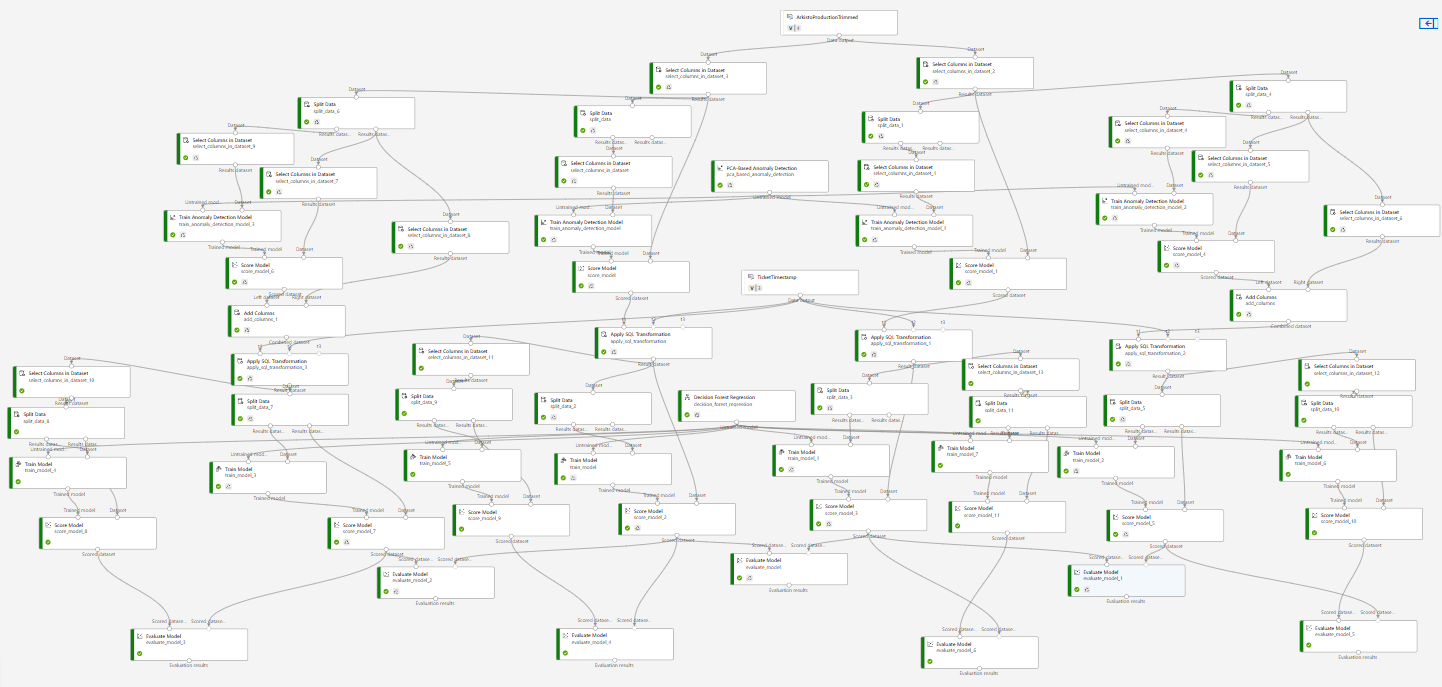
\includegraphics[width=150mm]{./appendices/pipeline-draft}
    \caption{Pipeline in all its glory
    \label{fig:pipeline draft}}
\end{figure}


%% ............................................................................................................


%% TODO: Mention that data splits in phase 1 have to be un-random
%% Otherwise, possible anomaly values used in phase 2 would be randomly included
%% Data in phase 1 need to be chronological!


%% TODO: Results: Feature Hashing runs out of memory in Model Training with full data (unconventional training)
%% Trying with smaller splits, which, once again, reduces data amount.

\begin{itcomment}
    Next in this subsection, ML studio pipeline used is explained in more detail.
    This means pictures about the pipeline,
    explanations about the components used and their parameters,
    etc. etc.

    Some of the content might be wise to move to the Results section.
    This needs more somewhat more thinking, also based on the results...
\end{itcomment}

%% TODO: unorganized text below!

%% TODO: Next up is outdated
%
%Usually <with usual ml methods> the estimates
%created using ML algorithms
%are formed based on the certain features
%presented on a one element of the data,
%or on one row.
%This means that in typical case,
%there is one column in the data
%given to the ML algorithm
%that is removed from the training data
%and this column value is what algorithm
%aims to predict.
%
%In this study case, however,
%data does not contain clear values
%that are being estimated
%and that can be used as comparison.
%
%\begin{tabular}{cccc}
%    LOG\_DATA \\
%    a=date & b=msg & c=\etc & \\
%    a & b & c & n1 \\
%    a & b & c & n2 \\
%    a & b & c & n3 \\
%    a & b & c & n4
%\end{tabular}
%
%\begin{tabular}{c}
%    EFECTE\_DATA \\
%    A YYYY.MM.DD hh:mm:ss \\
%    B YYYY.MM.DD hh:mm:ss \\
%    C YYYY.MM.DD hh:mm:ss \\
%    D YYYY.MM.DD hh:mm:ss \\
%    E YYYY.MM.DD hh:mm:ss
%\end{tabular}
%\\
%n1 = SUM(AB) \\
%n2 = SUM(C) \\
%n3 = SUM(DE) \\
%=> \\
%We could try to predict nx
%but usually this is done
%by making estimate based on
%a, b and c.
%Instead,
%we aim to estimate the sum of events
%in timeframe.
%We should also skip event instances
%that are close to each other
%to avoid counting multiple values
%linked to same error
%as different possible ticket creators.

%% ............................................................................................................

\subsubsection*{Memory issues and limitations}
Memory is crucial in ML training
as multiple steps happen
and data is formatted \etc. %% TODO: fix!
While building ML pipeline in Azure ML studio,
a memory issue emerged
that affected several components
and caused serious limitations
in terms of usable components and data size.
Due to the time limits of this study
this issue was not resolved
and the problem behind it was not found.
As several conditions
considering the environment costs
were already issued by the company,
the issue was declared to be linked with
compute instance property limitations.
However, this was not certain.

\todo{Limitations to components}
%% TODO: limitations to components
%% limitations to data size
%% effects on choises in components?

%% ............................................................................................................

\subsubsection*{Feature format for PCA-ADA}
%% TODO: n-gram vs pure data input
In Azure ML Studio
there is only one module selectable
for anomaly detecting,
the PCA-based anomaly detection module,
which is explained in section~\ref{subsec:bg-pca-ada}.
However,
with textual input like logs
it can be used at least in two ways.
First,
input data can be fed to
the algorithm trainer as is,
letting the PCA-based ADA component %% TODO: Explain ADA
do the work without further modifying the log rows.
This way,
the component tries to recognize the anomalies
based on all the information included in the row.
Practically this means
that the component processes data in textual format
making each row in the input
a feature as a whole
to consider.
\todo{PCA-ADA should be explained in background-section}

Second option is to
convert the textual features
into numerical n-gram features.
Each word or n-gram
is now a number of said instances found on
the row being processed,
and each row can be presented
as a sequence of numbers
indicating the number of those features.

%% TODO N-gram theory should be explained and referred properly. Here or in background!
N-grams can in addition have a weight
based on the frequency they appear
in the entire data.
Different weights usable in Azure ML component
are listed below.

\begin{enumerate}
    \item Binary Weight
    \item TF Weight
    \item IDF Weight
    \item TF-IDF Weight
\end{enumerate}

\todo{Explain different weights and open up more Azure ML Studio PCA-component}

%% TODO: RESULTS:
%   Pure n-gram feature component using skipped
%   Only 2% of the data could be used. Not enough.
%

%% ............................................................................................................

\subsubsection*{Anomaly probability}
%% TODO: PCA output
\begin{itcomment}
    Here we explain what PCA-component outputs and how the result is used in the pipeline.
\end{itcomment}

The output values of the PCA-ADA component are,
as explained in the section~\ref{subsec:bg-pca-ada},
normalized so the values range between 0 and 1.
This anomaly probability value
is the main output of hybrid ML phase 1.
Based on our initial hypothesis
that each anomalous event in the log
is linked to a real life support ticket received,
the bigger a single anomaly probability value is for a log row
the more likely that row is related to a ticket inducing event.


%% ............................................................................................................

\subsubsection*{Regression based estimating}
%% TODO: parameters?
%% Ticket amount forecasting
\begin{itcomment}
    Here is more information about different regression algorithms
    used in ML pipeline.
    Some basic information about all of them is given so the results are understandable
    by reader in the Result section.
\end{itcomment}

\begin{enumerate}
    \item Linear regression
    \item Decision forest regression
    \item \etc
    \item \etc
\end{enumerate}


\clearpage